\documentclass{article}
\usepackage[utf8]{inputenc}
\usepackage[spanish]{babel}
\usepackage{amsmath}
\usepackage{amssymb}
\usepackage{amsfonts}
\usepackage{hyperref}
\usepackage{textcomp}
\usepackage{graphicx}
\usepackage{pgfplots}
\usepackage{geometry}
\usepackage{tikz}
\usetikzlibrary{arrows, automata, positioning, quotes}
\hypersetup{
    colorlinks=true,
    linkcolor=black,
    citecolor=green,
    filecolor=magenta,      
    urlcolor=cyan,
}
\geometry{
  top=3cm,            % Margen superior
  bottom=3cm,         % Margen inferior
  left=3cm,           % Margen izquierdo
  right=3cm           % Margen derecho
}

\title{Estadística 1}
\author{Jorge Miguel Alvarado Reyes}
\date{16 Agosto 2023}

\setlength{\parindent}{0pt}
\begin{document}

\begin{titlepage}
    \begin{center}
        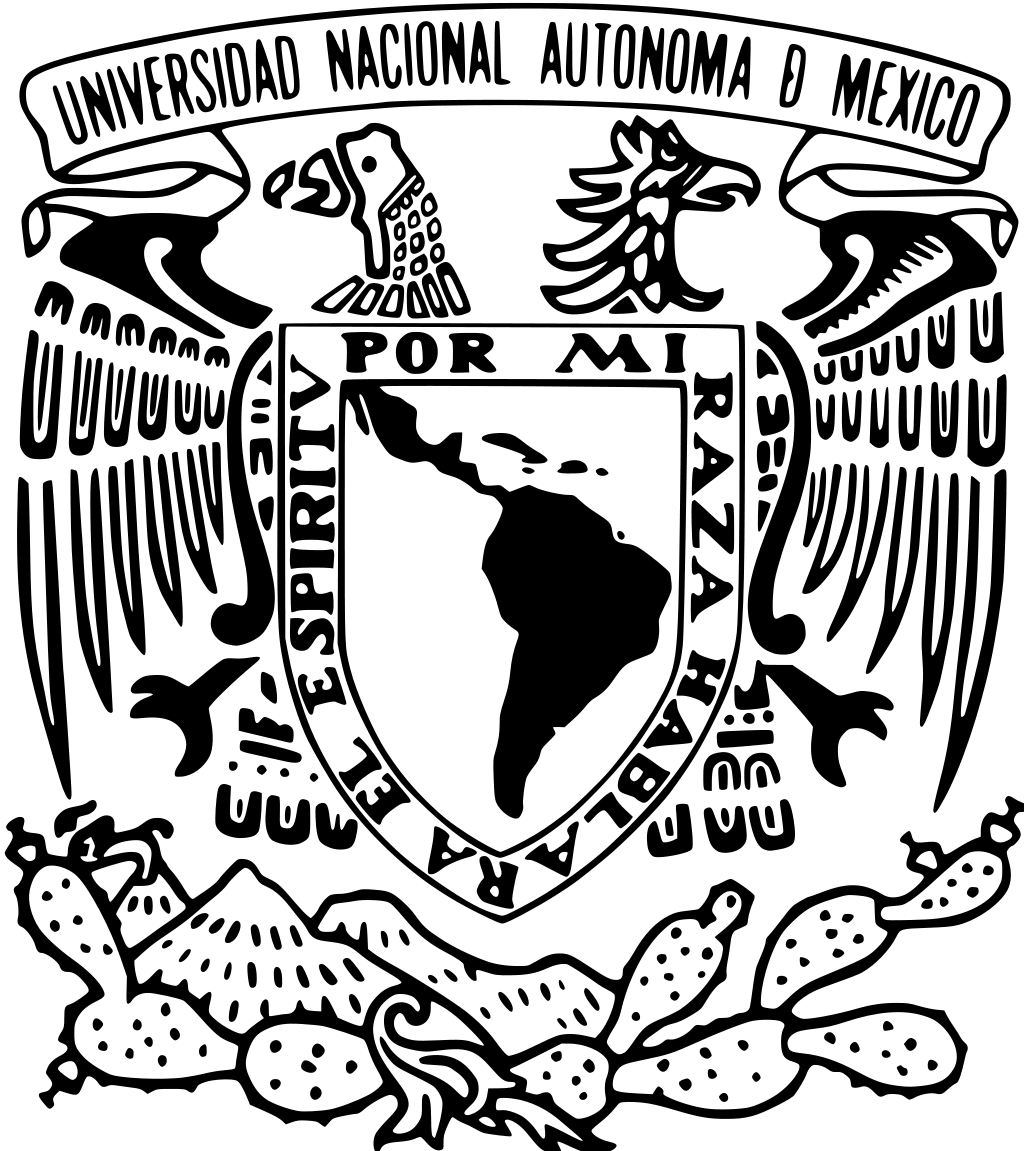
\includegraphics[width=0.2\textwidth]{../unam.png}
        \vspace*{.5cm}

        \LARGE
        \textbf{Universidad Nacional Autónoma de México}

        \vspace{0.5cm}
        \LARGE
        Facultad de Estudios Superiores Acatlán

        \vspace{2cm}

        \textbf{Apuntes} \\
        Procesos Estocasticos

        \vfill

        \vspace{1cm}

        \textbf{\large Autor:} \\
        Jorge Miguel Alvarado Reyes \\
        \vspace{.5cm}
        \normalsize \today

    \end{center}
\end{titlepage}
\newpage

\tableofcontents

\newpage

\section{29/01/2024}

\subsection{Contacto}

\begin{itemize}
    \item Numero: 5531185399
    \item Clave SEA: fvuzef
\end{itemize}

\subsection{Evaluacion}

\begin{itemize}
    \item 2 Examenes parciales 60\%
          \begin{itemize}
              \item 1er examen $\rightarrow$ viernes de la semana 9
              \item 2o examen $\rightarrow$ viernes de la semana 15
          \end{itemize}
    \item Tareas, Ejercicios, Practicas 20\%
    \item Proyecto final 20\%
          \begin{itemize}
              \item Paquete, software de 6 algoritmos que resuelvan cualquier proceso markoviano de decision
          \end{itemize}
\end{itemize}

\section{31/01/2024}

\subsection{Repaso de probabilidad}

\subsection{Espacio Muestral}

El espacio muestral, generalmente denotado por $S$, representa el conjunto completo de todos los posibles resultados individuales de un experimento aleatorio. Este conjunto puede ser finito o infinito, y los elementos dentro de él pueden ser numerables o no numerables. En esencia, el espacio muestral abarca todas las eventualidades que pueden surgir en un experimento, configurando así el universo de posibilidades a considerar en el análisis probabilístico.

\vspace{.25cm}

\subsection{Evento}

Un evento, en el contexto de la probabilidad, se refiere a cualquier subconjunto específico del espacio muestral. Esencialmente, es una colección de resultados del espacio muestral que comparten una o más características comunes. Los eventos son fundamentales en el estudio de la probabilidad, ya que representan los diferentes resultados que se pueden analizar y sobre los cuales se calculan las probabilidades.

\vspace{.25cm}

\subsection{Eventos mutuamente excluyentes}

Tambien llamados eventos disjuntos son aquellos que no tienen resultados en comun, es decir:

\[E_1 \cap E_2 = \emptyset\]

\subsection{Función de Probabilidad}

Sean \( S \) cualquier espacio muestral y \( E \) cualquier evento de este. Se llamará función de probabilidad sobre el espacio muestral \( S \) a \( P(E) \) si satisface los siguientes axiomas:

\begin{enumerate}
    \item \textbf{Axioma 1 (No negatividad):} Para cualquier evento \( E \) en \( S \), la probabilidad de \( E \) es siempre no negativa. Es decir, \( P(E) \geq 0 \).
    \item \textbf{Axioma 2 (Certidumbre):} La probabilidad del espacio muestral completo es 1. Es decir, \( P(S) = 1 \).
    \item \textbf{Axioma 3 (Aditividad):} Para cualquier secuencia de eventos mutuamente excluyentes \( E_1, E_2, E_3, \ldots \) en \( S \), la probabilidad de la unión de estos eventos es igual a la suma de sus probabilidades individuales. Es decir,
          \[ P\left(\bigcup_{i=1}^{\infty} E_i\right) = \sum_{i=1}^{\infty} P(E_i) \],
          siempre y cuando \( E_i \cap E_j = \emptyset \) para \( i \neq j \).
\end{enumerate}

\subsection{Probabilidad condicional}

La probabilidad condicional de un evento \( A \) dado que otro evento \( B \) ha ocurrido, denotada como \( P(A|B) \), se define como la probabilidad de que ocurra el evento \( A \) una vez que se sabe que \( B \) ha ocurrido. Esto se expresa matemáticamente por la fórmula:
\[ P(A|B) = \frac{P(A \cap B)}{P(B)} \]

donde:
\begin{itemize}
    \item \( P(A \cap B) \) es la probabilidad de que ocurran ambos eventos \( A \) y \( B \).
    \item \( P(B) \) es la probabilidad del evento \( B \).
\end{itemize}

Esta definición es válida siempre que \( P(B) > 0 \).

\textbf{Eventos independientes}

Dos eventos \( A \) y \( B \) en un espacio muestral \( S \) se consideran independientes si la ocurrencia de uno no afecta la probabilidad de ocurrencia del otro. Matemáticamente, esto se expresa diciendo que dos eventos \( A \) y \( B \) son independientes si y solo si:
\[ P(A \cap B) = P(A) \times P(B) \]

En otras palabras, la probabilidad de que ambos eventos ocurran juntos (la intersección de \( A \) y \( B \)) es igual al producto de sus probabilidades individuales. Si esta relación no se cumple, entonces los eventos se consideran dependientes.

\subsection{Ley multiplicativa de la probabilidad}

La ley multiplicativa de la probabilidad se utiliza para calcular la probabilidad de la intersección de dos eventos. Si tenemos dos eventos \( A \) y \( B \), la probabilidad de que ambos \( A \) y \( B \) ocurran, denotada como \( P(A \cap B) \), se calcula como:
\[ P(A \cap B) = P(A) \times P(B|A) \]
si \( P(A) > 0 \).

De manera alternativa, si \( P(B) > 0 \), se puede calcular como:
\[ P(A \cap B) = P(B) \times P(A|B) \]

Esta ley es una extensión de la definición de probabilidad condicional y es crucial en el cálculo de probabilidades para eventos dependientes.

\subsection{Variable aleatoria}


Una variable aleatoria es una función que asigna un valor numérico a cada resultado en un espacio muestral. Se denota comúnmente con letras mayúsculas, como \( X \), \( Y \), etc. Hay dos tipos principales de variables aleatorias:

\begin{itemize}
    \item \textbf{Variable Aleatoria Discreta:} Toma un número finito o contablemente infinito de valores distintos. La función de probabilidad de una variable aleatoria discreta, denominada función de masa de probabilidad (fmp), asigna una probabilidad a cada valor posible de la variable.
    \item \textbf{Variable Aleatoria Continua:} Toma un número infinito de posibles valores. La función de probabilidad de una variable aleatoria continua, conocida como función de densidad de probabilidad (fdp), asigna probabilidades a intervalos de valores.
\end{itemize}

La variable aleatoria es fundamental en el estudio de la probabilidad, ya que proporciona el enlace entre los eventos aleatorios y los análisis numéricos.

\subsection{Distribucion de probabilidad}

La función de probabilidad de una Variable Aleatoria (V.A) describe cómo se asignan las probabilidades a los diferentes valores que la V.A puede tomar. Esta función varía según si la V.A es discreta o continua:

\begin{itemize}
    \item \textbf{Para una V.A Discreta:} La función de probabilidad es la función de masa de probabilidad (fmp), que proporciona la probabilidad para cada valor posible que la variable aleatoria puede asumir. La fmp \( f(x) \) satisface dos propiedades:
          \begin{enumerate}
              \item \( f(x) \geq 0 \) para todo \( x \).
              \item La suma de \( f(x) \) sobre todos los posibles valores de \( x \) es igual a 1.
          \end{enumerate}
    \item \textbf{Para una V.A Continua:} La función de probabilidad es la función de densidad de probabilidad (fdp), que asigna probabilidades a intervalos de valores de la V.A. La fdp \( f(x) \) cumple con:
          \begin{enumerate}
              \item \( f(x) \geq 0 \) para todo \( x \).
              \item La integral de \( f(x) \) sobre todo el espacio es igual a 1.
          \end{enumerate}
\end{itemize}

Estas funciones son fundamentales para comprender la naturaleza y el comportamiento de las variables aleatorias en el estudio de la probabilidad y estadística.

\textbf{Resumen}

\begin{itemize}
    \item \textbf{Función de Probabilidad de v.a \( X \)}: \( p(x) = P(X=x) \). Esta función asigna la probabilidad de que la variable aleatoria \( X \) tome un valor específico \( x \).

    \item \textbf{Función de Probabilidad de un Evento \( A \)}: \( P(A) \). Representa la probabilidad de que ocurra el evento \( A \).

    \item \textbf{Distribución de Probabilidad de v.a \( X \)}: Describe cómo se distribuyen las probabilidades a través de los diferentes valores que puede tomar la variable aleatoria \( X \). Se diferencia en distribuciones discretas y continuas.

    \item \textbf{Función de Distribución Acumulada}: Proporciona la probabilidad acumulativa de que la variable aleatoria \( X \) sea menor o igual a un valor específico. Se representa como \( F(x) = P(X \leq x) \) y varía para variables aleatorias discretas y continuas.
\end{itemize}

\section{02/02/2024}

\subsection{Repaso de probabilidad}

\subsection{Distribuciones discretas}

\begin{itemize}
    \item \textbf{Uniforme Discreta}: Esta distribución asigna la misma probabilidad a cada uno de los $n$ resultados diferentes en un espacio de muestra finito. La función de masa de probabilidad (PMF) es $P(X = x) = \frac{1}{n}$ para $x = 1, 2, \ldots, n$.

    \item \textbf{Bernoulli}: Modela experimentos que tienen exactamente dos resultados posibles, "éxito" (con probabilidad $p$) y "fracaso" (con probabilidad $1-p$). La PMF es $P(X = x) = p^x(1-p)^{1-x}$ para $x = 0, 1$.

    \item \textbf{Binomial}: Extiende la distribución de Bernoulli a $n$ ensayos independientes, con $p$ siendo la probabilidad de éxito en cada ensayo. La PMF es $P(X = k) = \binom{n}{k}p^k(1-p)^{n-k}$ para $k = 0, 1, \ldots, n$.

    \item \textbf{Geométrica}: Mide el número de ensayos necesarios para obtener el primer éxito. La PMF es $P(X = k) = (1-p)^{k-1}p$ para $k = 1, 2, \ldots$.

    \item \textbf{Binomial Negativa o de Pascal}: Cuenta el número de ensayos requeridos para obtener un número fijo $r$ de éxitos. La PMF es $P(X = k) = \binom{k-1}{r-1}p^r(1-p)^{k-r}$ para $k = r, r+1, \ldots$.

    \item \textbf{Hipergeométrica}: Modela el número de éxitos en una muestra sin reemplazo. La PMF es $P(X = k) = \frac{\binom{K}{k}\binom{N-K}{n-k}}{\binom{N}{n}}$, donde $N$ es el tamaño de la población, $K$ es el número total de éxitos en la población, y $n$ es el tamaño de la muestra.

    \item \textbf{Poisson}: Modela el número de eventos en un intervalo fijo de tiempo o espacio. La PMF es $P(X = k) = \frac{\lambda^k e^{-\lambda}}{k!}$ para $k = 0, 1, 2, \ldots$, donde $\lambda$ es el número promedio de eventos en el intervalo.
\end{itemize}

\subsection{Esperanza matematica de distribuciones discretas}

Sea x una variable aleatrois discreta con funcion de probabilidad $(p(x))$ entonces el valor esperado de $x$, $E(x)$ está definido por

\[E(X) = \sum xp(x)\]

Regularmente asociamos la esperanza con la media poblacional $\mu$

\subsection{Variana de una variable aleatoria discreta}

Se define como el valor esperado de $(X - \mu)^2$ es decir
\[V(X) = E((X-\mu)^2)\]

\subsection{Distribuciones continuas}

\begin{itemize}
    \item \textbf{Uniforme}: La distribución uniforme continua describe un experimento donde todos los resultados en un intervalo \([a, b]\) son igualmente probables. Su función de densidad es $f(x) = \frac{1}{b-a}$ para $x \in [a, b]$. La media es $\mu = \frac{a+b}{2}$ y la varianza es $\sigma^2 = \frac{(b-a)^2}{12}$.

    \item \textbf{Normal}: También conocida como la distribución Gaussiana, caracterizada por su función de densidad en forma de campana $f(x) = \frac{1}{\sigma\sqrt{2\pi}}e^{-\frac{1}{2}(\frac{x-\mu}{\sigma})^2}$, donde $\mu$ es la media y $\sigma$ es la desviación estándar. Es fundamental en teoría de probabilidad y estadística debido a su propiedad de regresión al promedio y el Teorema del Límite Central.

    \item \textbf{Exponencial}: Modela el tiempo entre eventos en un proceso de Poisson, con tasa de ocurrencia $\lambda$. Su función de densidad es $f(x) = \lambda e^{-\lambda x}$ para $x \geq 0$. La media y la varianza son $\frac{1}{\lambda}$.

    \item \textbf{Gamma}: Generaliza las distribuciones exponencial y $\chi^2$, útil para modelar tiempos de espera para múltiples eventos. Su función de densidad es $f(x) = \frac{x^{k-1}e^{-x/\theta}}{\theta^k \Gamma(k)}$ para $x > 0$, donde $k$ es el parámetro de forma y $\theta$ el parámetro de escala.

    \item \textbf{Beta}: Modela variables aleatorias que toman valores entre 0 y 1, útil para modelar proporciones. Su función de densidad es $f(x) = \frac{x^{\alpha-1}(1-x)^{\beta-1}}{B(\alpha, \beta)}$ para $0 < x < 1$, donde $\alpha$ y $\beta$ son parámetros de forma.

    \item \textbf{Triangular}: Una distribución simple definida por un mínimo, un máximo, y un valor modal. Su función de densidad cambia linealmente entre estos puntos. Es útil para simulaciones y modelado de fenómenos con un conocimiento limitado.

    \item \textbf{Weibull}: Extiende la distribución exponencial para permitir una tasa de fallo variable. Su función de densidad es $f(x) = \frac{k}{\lambda} \left( \frac{x}{\lambda} \right)^{k-1} e^{-(x/\lambda)^k}$ para $x \geq 0$, donde $k$ es el parámetro de forma y $\lambda$ el de escala. Es muy utilizada en análisis de confiabilidad y duración de vida.
\end{itemize}

\subsection{Esperanza matematica de distribuciones continuas}

Sea x una variable aleatoria continua

\section*{Resumen Probabilidad}

En teoría de probabilidad, las variables aleatorias se clasifican en continuas o discretas, y cada una tiene asociada una función de densidad o una función de distribución acumulativa, respectivamente.

\subsection*{Variables Aleatorias Discretas}

Para una variable aleatoria discreta \(X\), la función de probabilidad, también conocida como función de masa de probabilidad (PMF), se denota por \(p(x)\) y se define como:

\[ p(x) = P(X = x) \]

donde \(P(X = x)\) es la probabilidad de que \(X\) tome el valor \(x\).

La función de distribución acumulativa (CDF), \(F(x)\), para una variable aleatoria discreta se define como la probabilidad de que \(X\) tome un valor menor o igual a \(x\):

\[ F(x) = P(X \leq x) = \sum_{x_i \leq x} p(x_i) \]

\subsection*{Variables Aleatorias Continuas}

Para una variable aleatoria continua \(X\), la función de densidad de probabilidad (PDF) se denota por \(f(x)\) y satisface:

\[ f(x) \geq 0 \]

\[ \int_{-\infty}^{\infty} f(x) \, dx = 1 \]

La PDF describe la densidad de probabilidad en cada punto de la línea real.

La función de distribución acumulativa (CDF), \(F(x)\), para una variable aleatoria continua se define como la probabilidad de que \(X\) sea menor o igual a \(x\):

\[ F(x) = P(X \leq x) = \int_{-\infty}^{x} f(t) \, dt \]

La CDF es una función no decreciente que se aproxima a 0 a medida que \(x\) se aproxima a \(-\infty\) y se aproxima a 1 a medida que \(x\) se aproxima a \(\infty\).

\section{07/02/2024}


\subsection{Unidad 1. Elementos de procesos estocásticos}

\textbf{Definición de procesos estocásticos}

La primera idea basica es identificar a un proceso estocastico como una sucesion de variables aleatorias ${X_n; n \in \mathbb{N}}$ donde el subindice indica el instante de tiempo o espacio correspondiente. la idea puede generalizarse de manera que los instantes de tiempo desan continuos donde  ${X_t;t \in \mathbb{R}} $

\textbf{Conjunto de estados}

Se denomina conjunto de estados $S$, al conjunto de los posibles valores que pueden tomar las variables aleatorias


\textbf{Conjunto parametrico}

Se denomina conjunto parametrico $T$, al conjunto de subindices que puede tomar $t$\\
Al igual que en las variables aleatorias, este conjunto puede ser discreto o continuo

\textbf{Ejemplo}

Se lanza una moneda varias veces, supongase que cada vez que sale cara un jugador gana 1 dolar y cada vez que sale ruz pierde un dolar. Defina lo anterior como un proceso estocastico planteando el conjunto de estados, el conjunto parametico y la forma en que se definirian las probabilidades

$X_t$: Ganancia o perdida en el t-esimo lanzamiento de la moneda

$S = \{\dots, -3,-2,-1, 0, 1, 2, 3, \dots\}$

$T = \{1,2,3,\dots\}$

Si fijo el parametro, $t = 3$

Podemos hacer realizaciones: $(t,t,c)$

Ver como se modifica el conjunto de estados

\section{09/02/2024}

\subsection{Clasificacion de los prcesos estocasticos}

Se subdividen dependiendo de acuerdo a la estructurra de los conjuntos $S$ y $T$.

De a cuerdo a las caracteristicas probabilisticas de la variable aleatoria $X_t$

\newpage

\section{Proceso de Bernoulli}

Un proceso estocástico $\{X_n; n \in \mathbb{N}\}$ se denomina proceso de Bernoulli si cumple con las siguientes condiciones:

\begin{itemize}
    \item Las variables aleatorias $X_1, X_2, \ldots$ son mutuamente independientes.
    \item Cada variable aleatoria $X_n$ sigue una distribución de Bernoulli, donde la probabilidad de éxito (denotado por $X_n = 1$) es $p$, y la probabilidad de fracaso (denotado por $X_n = 0$) es $1-p$, que también podemos denotar por $q$. Es decir:
          \begin{align*}
              \mathbb{P}(X_n = 1) & = p,       \\
              \mathbb{P}(X_n = 0) & = 1-p = q.
          \end{align*}
\end{itemize}

En este contexto, al evento $X_n = 1$ lo llamamos \textit{éxito} y al evento $X_n = 0$, \textit{fracaso}.

Sea $\{X_n; n \in \mathbb{N}\}$ un proceso de Bernoulli con probabilidad de éxito $p$. Definimos $S_n$ como el número total de éxitos en los primeros $n$ ensayos. Es decir, $S_n$ se define como:

\[
    S_n = \sum_{i=1}^{n} X_i,
\]

Tambien lo encontramos como:

\[
    N_t =
    \begin{cases}
        0                       & \text{si } n=0           \\
        X_1 + X_2 + \dots + X_n & \text{si } n=1,2,3,\dots
    \end{cases}
\]


donde cada $X_i$ es una variable aleatoria que indica el éxito ($X_i = 1$) o fracaso ($X_i = 0$) en el $i$-ésimo ensayo. Por lo tanto, $S_n$ sigue una distribución binomial con parámetros $n$ y $p$, lo cual se puede expresar como:

\[
    S_n \sim \text{Bin}(n, p),
\]

donde la probabilidad de obtener exactamente $k$ éxitos en $n$ ensayos está dada por la función de probabilidad:

\[
    P(S_n = k) = \binom{n}{k} p^k q^{n-k},
\]

para $k = 0, 1, 2, \ldots, n$.

La esperanza (valor esperado) y la varianza de $S_n$, donde $S_n \sim \text{Bin}(n, p)$, se pueden calcular de la siguiente manera:

\begin{itemize}
    \item \textbf{Esperanza:} La esperanza de $S_n$ indica el número promedio de éxitos en $n$ ensayos y se calcula como
          \[
              \mathbb{E}[S_n] = np.
          \]

    \item \textbf{Varianza:} La varianza de $S_n$ mide la dispersión de los éxitos alrededor de la esperanza y se calcula como
          \[
              \text{Var}(S_n) = np(1-p) = npq.
          \]
\end{itemize}

Estas fórmulas nos permiten entender las propiedades estadísticas del número de éxitos en un proceso de Bernoulli.

\section{Caminata Aleatoria Simple}

Una \textit{caminata aleatoria simple} sobre el conjunto de los enteros es un proceso estocástico a tiempo discreto $\{X_n: n \in \mathbb{Z}^{+}\}$, donde $\mathbb{Z}^{+}$ representa los enteros positivos incluyendo el cero. Iniciando en el estado 0, el proceso se define de tal manera que, en cada paso $n$, el proceso puede moverse al estado $i+1$ con una probabilidad $p$ o al estado $i-1$ con una probabilidad $q$, donde $i$ es el estado actual y $p + q = 1$.

El valor de $X_n$ representa la posición del proceso en el tiempo $n$. La regla de transición se aplica de manera idéntica en cada paso, independientemente de la posición actual, lo que implica que la caminata tiene la propiedad de incrementos independientes e idénticamente distribuidos (i.i.d.).

Las probabilidades de transición válidas para cualquier $n \geq 0$, y para cualquier par de enteros $i$ y $j$, se expresan como:

\[
    P(X_{n+1} = j | X_n = i) =
    \begin{cases}
        p, & \text{si } j = i + 1,   \\
        q, & \text{si } j = i - 1,   \\
        0, & \text{de lo contrario}.
    \end{cases}
\]

Esto significa que la probabilidad de moverse de un estado $i$ a un estado $j$ en el siguiente paso depende únicamente de si $j$ es inmediatamente adyacente a $i$ y se ajusta a la regla de que $p + q = 1$.

\vspace*{.2cm}

Dado que estas probabilidades no dependen de $n$, se dice que son homogéneas en el tiempo, es decir, son las mismas para cualquier valor de $n$. A partir de estas consideraciones, se dice que este proceso cumple con la propiedad de Markov; es decir, el estado futuro del proceso depende únicamente del estado presente y no de los estados previos.

\subsection*{Definición Formal de una Caminata Aleatoria}

Sean $\{\epsilon_i\}_{i=1}^{\infty}$ una sucesión de variables aleatorias independientes e idénticamente distribuidas tales que $\mathbb{P}(\epsilon_i = 1) = p$ y $\mathbb{P}(\epsilon_i = -1) = q$, donde $p + q = 1$. Entonces, para $n \geq 1$, se define $X_n = X_0 + \epsilon_1 + \epsilon_2 + \dots + \epsilon_n$. Sin pérdida de generalidad, supondremos que $X_0 = 0$, lo que implica que el proceso inicia en el origen. Por lo tanto, la posición en el tiempo $n$ está dada por la suma de los incrementos individuales representados por las variables $\epsilon_i$.

De esta manera, la caminata aleatoria se puede representar como:

\[
    X_n = \sum_{i=1}^{n} \epsilon_i.
\]

Cada $\epsilon_i$ toma el valor de 1 o -1, correspondiendo a un paso hacia la derecha o hacia la izquierda, respectivamente, en la línea de los enteros.

\subsection*{Esperanza de $X_n$}

La esperanza de $X_n$ se calcula como sigue:

\[
    \mathbb{E}[X_n] = \mathbb{E}\left[\sum_{i=1}^{n} \epsilon_i\right] = \sum_{i=1}^{n} \mathbb{E}[\epsilon_i].
\]

Dado que cada $\epsilon_i$ tiene una distribución con $\mathbb{P}(\epsilon_i = 1) = p$ y $\mathbb{P}(\epsilon_i = -1) = q$, la esperanza de $\epsilon_i$ es:

\[
    \mathbb{E}[\epsilon_i] = 1\cdot p + (-1)\cdot q = p - q.
\]

Por lo tanto, la esperanza de $X_n$ es:

\[
    \mathbb{E}[X_n] = n(p - q).
\]

\subsection*{Varianza de $X_n$}

La varianza de $X_n$ se puede calcular utilizando la propiedad de la varianza de sumas de variables aleatorias independientes:

\[
    \text{Var}(X_n) = \text{Var}\left(\sum_{i=1}^{n} \epsilon_i\right) = \sum_{i=1}^{n} \text{Var}(\epsilon_i).
\]

La varianza de cada $\epsilon_i$ es:

\[
    \text{Var}(\epsilon_i) = \mathbb{E}[\epsilon_i^2] - (\mathbb{E}[\epsilon_i])^2.
\]

Ya que $\epsilon_i^2 = 1$ para $\epsilon_i = 1$ o $\epsilon_i = -1$, tenemos $\mathbb{E}[\epsilon_i^2] = 1$. Por lo tanto:

\[
    \text{Var}(\epsilon_i) = 1 - (p - q)^2 = 1 - (p^2 + q^2 - 2pq) = 1 - (p^2 + (1-p)^2 - 2p(1-p)).
\]

Simplificando, obtenemos:

\[
    \text{Var}(\epsilon_i) = 4pq.
\]

Finalmente, la varianza de $X_n$ es:

\[
    \text{Var}(X_n) = n \cdot 4pq.
\]

\subsection*{Probabilidades de Transición}

Suponiendo que la caminata aleatoria inicia en 0, es fácil deducir que después de efectuar un número par de pasos, la cadena solo puede terminar en posiciones pares, y si se efectúa un número impar de pasos, la posición final debe ser impar. Además, sabemos que después de efectuar $n$ pasos, la caminata solo puede llegar a una distancia máxima de $n$ unidades a la izquierda o a la derecha del origen.

Teniendo esto como base, definiremos las probabilidades de transición para cualesquiera números enteros $x$ y $y$, tales que $-n \leq x \leq n$ y para el caso cuando $x$ y $n$ son ambos pares o ambos impares, la probabilidad de transición de la posición $x$ a la posición $y$ en $n$ pasos, denotada por $P\{X_n = x | X_0 = X_0\}$, es dada por:

\[
    P\{X_n = x | X_0 = X_0\} = \binom{n}{\frac{n + x}{2}} p^{\frac{n + x}{2}} q^{\frac{n - x}{2}},
\]

\[
    P\{X_n = x | X_0 = y\} = \binom{n}{\frac{n + x - y}{2}} p^{\frac{n + x - y}{2}} q^{\frac{n - x + y}{2}},
\]

donde $\binom{n}{k}$ es el coeficiente binomial que representa el número de formas de elegir $k$ elementos de un total de $n$ elementos, y se asume que $p + q = 1$. Esta fórmula es válida bajo la condición de que tanto $(n + y - x)$ como $(n - y + x)$ sean no negativos y pares, lo cual asegura que los exponentes de $p$ y $q$ sean enteros no negativos. En cualquier otro caso, $P_{x,y}^{(n)} = 0$, reflejando la imposibilidad de moverse una cantidad impar de posiciones en un número par de pasos, y viceversa.

\subsection*{Ejemplo}

Considere una partícula que realiza una caminata aleatoria simétrica.

\begin{itemize}
    \item \textbf{Encuentre todas las posibles secuencias de movimiento de la partícula en una
              caminata de 4 pasos, indicando la posición final en la que se encuentra la
              partícula al realizar cada una de las secuencias posibles.}

          Para una caminata de 4 pasos, cada paso puede ser hacia la derecha (+1) o hacia la izquierda (-1). Las posibles secuencias de 4 pasos y sus posiciones finales son:

          \begin{tabular}{c|c}
              Secuencia & Posición Final \\
              \hline
              ++++      & 4              \\
              +++-      & 2              \\
              ++-+      & 2              \\
              ++--      & 0              \\
              +-++      & 2              \\
              +-+-      & 0              \\
              +--+      & 0              \\
              +---      & -2             \\
              -+++      & 2              \\
              -++-      & 0              \\
              -+-+      & 0              \\
              -+--      & -2             \\
              --++      & 0              \\
              --+-      & -2             \\
              ---+      & -2             \\
              ----      & -4             \\
          \end{tabular}

    \item \textbf{¿Con qué probabilidad ocurre cada una de estas secuencias?}

          Dado que la caminata es simétrica, cada paso tiene una probabilidad de $1/2$. La probabilidad de cualquier secuencia específica de 4 pasos es entonces $(1/2)^4 = 1/16$.

    \item \textbf{¿Con qué probabilidad termina la partícula en cada posición?}

          \begin{itemize}
              \item $\mathbb{P}(X_4 = 4) = \frac{1}{16}$
              \item $\mathbb{P}(X_4 = 2) = \frac{4}{16}$
              \item $\mathbb{P}(X_4 = 0) = \frac{6}{16}$
              \item $\mathbb{P}(X_4 = -2) = \frac{4}{16}$
              \item $\mathbb{P}(X_4 = -4) = \frac{1}{16}$
          \end{itemize}

    \item \textbf{¿Cuál es el valor medio de la posición final \( X \)?}

          El valor medio de la posición final, o el valor esperado \( \mathbb{E}[X] \), para una caminata aleatoria simétrica de 4 pasos se calcula como la suma de las posiciones finales multiplicadas por sus respectivas probabilidades. En este caso, \( \mathbb{E}[X] = 0 \), ya que la caminata es simétrica y las posiciones finales positivas y negativas se equilibran entre sí.
\end{itemize}

\subsection*{Ejemplo}

Una partícula realiza una caminata aleatoria sobre los enteros comenzando en la posición 4. Se desea encontrar la probabilidad de que la partícula se encuentre en la posición 5 después de 7 pasos, con una probabilidad de moverse hacia la derecha del 75\%.

\[
    P\{X_7 = 5 | X_0 = 4\} = \binom{7}{\frac{7 + 5 - 4}{2}} p^{\frac{7 + 5 - 4}{2}} q^{\frac{7 - 5 + 4}{2}},
\]

\[
    P\{X_7 = 5 | X_0 = 4\} = \binom{7}{4} (0.75)^{4} (0.25)^{3} = 0.173
\]

\newpage

\section{El Problema del Jugador}

Consideramos un caso particular de una caminata aleatoria, donde un jugador \(A\) apuesta sucesivamente una unidad monetaria contra otro jugador \(B\). El capital inicial para cada jugador es \(k\) y \(n-k\) respectivamente, lo que implica que hay un capital total igual a \(N\). En cada apuesta, \(A\) tiene una probabilidad \(p\) de ganar y una probabilidad \(q\) de perder, asumiendo que \(p + q = 1\) y que no hay empates. Denotemos por \(X_n\) la fortuna del jugador \(A\) al tiempo \(n\), de manera que se modela como una caminata aleatoria que inicia en el estado \(k\) y eventualmente puede terminar en uno de los estados absorbentes \(0\) o \(N\).

\vspace{.25cm}

Estos dos estados, \(0\) y \(N\), son denominados estados absorbentes ya que, una vez alcanzados, el juego termina. La caminata aleatoria representada por \(X_n\) ofrece un marco para analizar la evolución del capital de \(A\) a través del tiempo hasta que se alcance uno de estos estados absorbentes.

\vspace{.25cm}

Regularmente, en este escenario la pregunta típica es: ¿Cuál es la probabilidad de que eventualmente el jugador \( A \) se arruine? Por tal motivo a este problema se le llama \textbf{Problema de la Ruina del Jugador}.

\vspace{.25cm}

Sea \( \gamma \) el primer momento en el que la caminata aleatoria visita alguno de los 2 estados absorbentes, es decir, \( \gamma = \min\{n \geq 0 \mid X_n = 0 \text{ o } X_n = N\} \). La probabilidad de ruina a partir de tener \( k \) unidades monetarias es una probabilidad condicional que se plantea como:

\[ U_k = P(X_\gamma = 0 \mid X_0 = k) \]

\subsection*{Definición}


La probabilidad de ruina del jugador \( A \), a partir de tener \( k \) unidades monetarias es:

\[
    U_k =
    \begin{cases}
        \frac{N - k}{N}                                                                                & \text{si } p = q = \frac{1}{2},                       \\[10pt]
        \frac{\left(\frac{q}{p}\right)^k - \left(\frac{q}{p}\right)^N}{1 - \left(\frac{q}{p}\right)^N} & \text{si } p \neq q \text{ y } p, q \neq \frac{1}{2}.
    \end{cases}
\]

\subsection*{Número Esperado de Apuestas}

Sea \( m_k \) el número esperado de apuestas antes de que termine el juego, en donde el jugador A tiene un capital inicial de \( k \) unidades y B tiene \( N-k \). Así:

\[
    m_k =
    \begin{cases}
        K(N-K)                                                                                                          & \text{si } p = q = \frac{1}{2},                       \\[10pt]
        \frac{1}{q-p}\left( K - N\left(\frac{1-\left(\frac{q}{p}\right)^K}{1-\left(\frac{q}{p}\right)^N}\right) \right) & \text{si } p \neq q \text{ y } p, q \neq \frac{1}{2}.
    \end{cases}
\]

\newpage

\subsection*{Ejemplos}

\subsubsection*{¿Cuál es la probabilidad de que un jugador se arruine si comenzó jugando con 5 pesos y el jugador contrario con 12, lanzando para tales efectos una moneda, donde si sale cruz el jugador gana 1 peso y si sale cara el jugador pierde 1 peso?}

\subsubsection*{Datos Disponibles}
\begin{itemize}
    \item Capital inicial del jugador A (\(k\)): 5 pesos.
    \item Capital total (\(N\)): \(k\) (del jugador A) + capital del jugador B = \(5 + 12 = 17\) pesos.
    \item Probabilidades de ganar (\(p\)) y perder (\(q\)): \(0.5\), ya que es una moneda justa.
\end{itemize}

\subsubsection*{Fórmulas a Utilizar}
Para calcular la probabilidad de ruina del jugador A (\(U_k\)), usamos la fórmula:
\[ U_k = \frac{N - k}{N} \]

\subsubsection*{Sustitución y Cálculo}
Sustituyendo \(k = 5\) y \(N = 17\) en la fórmula, obtenemos:
\[ U_5 = \frac{17 - 5}{17} = \frac{12}{17} \]

Realizando el cálculo, encontramos que:
\[ U_5 = 0.7058823529411765 \]

Por lo tanto, la probabilidad de que el jugador se arruine es aproximadamente \(70.6\%\).

\vspace{0.25cm}

\textbf{¿Qué sucede si la moneda está cargada a favor del jugador A con un 63\%?}

\subsubsection*{Datos Disponibles}
\begin{itemize}
    \item Capital inicial del jugador A (\(k\)): 5 pesos.
    \item Capital total (\(N\)): 17 pesos.
    \item Probabilidad de ganar (\(p\)): \(0.63\) (moneda cargada a favor del jugador A).
    \item Probabilidad de perder (\(q\)): \(0.37\) (resultado de \(1 - p\)).
\end{itemize}

\subsubsection*{Fórmula a Utilizar}
Para calcular la probabilidad de ruina del jugador A (\(U_k\)) con una moneda cargada, usamos la fórmula:
\[ U_k = \frac{\left(\frac{q}{p}\right)^k - \left(\frac{q}{p}\right)^N}{1 - \left(\frac{q}{p}\right)^N} \]

\subsubsection*{Sustitución y Cálculo}
Sustituyendo los valores de \(p = 0.63\), \(q = 0.37\), \(k = 5\) y \(N = 17\) en la fórmula, obtenemos:
\[ U_5 = \frac{\left(\frac{0.37}{0.63}\right)^5 - \left(\frac{0.37}{0.63}\right)^{17}}{1 - \left(\frac{0.37}{0.63}\right)^{17}} \]

Realizando el cálculo, encontramos que la probabilidad de ruina del jugador A es aproximadamente \(0.070\) o \(7.0\%\).

Por lo tanto, con la moneda cargada a favor, la probabilidad de que el jugador A se arruine disminuye significativamente.

\vspace{0.25cm}

\textbf{¿Cuál es el número esperado de apuestas antes de la ruina para ambos casos?}

\subsubsection*{Caso de Moneda Justa (\(p = q = 0.5\))}
Para el caso de una moneda justa, el número esperado de apuestas antes de la ruina, \(m_k\), se calcula como:
\[ m_k = k(N-k) \]
donde \(k = 5\) y \(N = 17\).

Sustituyendo los valores, obtenemos:
\[ m_k = 5(17-5) = 60 \]
Por lo tanto, el número esperado de apuestas antes de la ruina del jugador A con una moneda justa es de \textbf{60} apuestas.

\subsubsection*{Caso de Moneda Cargada (\(p = 0.63\), \(q = 0.37\))}
Para el caso de una moneda cargada a favor del jugador A, el número esperado de apuestas antes de la ruina, \(m_k\), se calcula como:
\[ m_k = \frac{1}{q-p}\left( k - N\left(\frac{1-\left(\frac{q}{p}\right)^k}{1-\left(\frac{q}{p}\right)^N}\right) \right) \]
donde \(k = 5\), \(N = 17\), \(p = 0.63\) y \(q = 0.37\).

Sustituyendo los valores, obtenemos:
\[ m_k = \frac{1}{0.37-0.63}\left( 5 - 17\left(\frac{1-\left(\frac{0.37}{0.63}\right)^5}{1-\left(\frac{0.37}{0.63}\right)^{17}}\right) \right) \]
\[ m_k \approx 41.59 \]
Por lo tanto, el número esperado de apuestas antes de la ruina del jugador A con una moneda cargada es aproximadamente \textbf{41.59} apuestas.

\newpage

\section{Cadenas de Markov}

Objetivo: El alumno explicará las cadenas de Markov, sus propiedades de transición en una y varias unidades de tiempo, las ecuaciones de Chapman-Kolmogorov, el análisis matricial de estas probabilidades, y las clasificaciones de los estados utilizando la teoría de grafos. Asimismo, se abordará el comportamiento asintótico con el fin de aplicar estos conceptos a casos básicos.

\vspace{.25cm}

En términos intuitivos, una cadena de Markov es un tipo de proceso estocástico que posee un número finito de estados. Las probabilidades de transición a cada estado dependen únicamente del estado actual, no de la secuencia de eventos que condujo a él.

\subsection*{Definición}
Un proceso estocástico \( X_t \) tiene la propiedad de Markov si y solo si la probabilidad de transitar al estado \( j \) en el tiempo \( t+1 \), dado el estado actual \( i \) en el tiempo \( t \), es independiente de la trayectoria pasada. Esto se expresa matemáticamente como:
\[ P(X_{t+1} = j | X_0 = k_0, X_1 = k_1, \ldots, X_{t-1} = k_{t-1}, X_t = i) = P(X_{t+1} = j | X_t = i) \]
para \( t = 0, 1, 2, \ldots \).

Esta propiedad, conocida como la propiedad Markoviana, establece que la probabilidad condicional de cualquier evento futuro, dados los eventos pasados y el estado actual, es independiente de los eventos pasados y depende únicamente del estado presente.

\subsection*{Definición}
Un proceso estocástico es una \textit{cadena de Markov} si satisface la propiedad Markoviana.

\subsection{Probabilidades de Transición}

Las probabilidades condicionales \( P(X_{t+1} = j | X_t = i) \) en una cadena de Markov se llaman probabilidades de transición (de un paso).

Si para cada \( i \) y \( j \), se cumple que \( P(X_{t+1} = j | X_t = i) = P(X_1 = j | X_0 = i) \) para todo \( t \geq 1 \), entonces se dice que las probabilidades de transición de un paso son estacionarias. Es decir, tener probabilidades de transición estacionarias implica que las probabilidades de transición no cambian con el tiempo.

Obsérvese además que la existencia de probabilidades de transición de un paso estacionarias, implica que para cada \( i \) y \( j \) y para todo \( n \geq 0 \), se tiene que
\[ P(X_{t+n} = j | X_t = i) = P(X_n = j | X_0 = i) \]
para todo \( t \geq 0 \).

A estas probabilidades de transición se les llama probabilidades de transición de \( n \) pasos.

\vspace{0.25cm}

Para simplificar la notación de las probabilidades de transición estacionarias, sea
\[ p_{ij} = P(X_{t+1} = j | X_t = i) \]
\[ p_{ij}^{(n)} = P(X_{t+n} = j | X_t = i) \]

Cuando \( n=1 \), observe que \( p_{ij}^{(1)} = p_{ij} \).

Cuando \( n=0 \), \( p_{ij}^{(0)} \) es \( P(X_0 = j | X_0 = i) \) que es igual a 1 cuando \( i=j \) y 0 en otro caso.

\newpage

Estas probabilidades, como cualquier otra, deben ser no negativas y, como el proceso debe hacer una transición a algún estado, deben satisfacer las siguientes propiedades:

\begin{enumerate}
    \item \( p_{ij}^{(n)} \geq 0 \) para todo \( i, j \) y \( n=0,1,2,\ldots \)
    \item \( \sum_{j=0}^{S} p_{ij}^{(n-1)} = 1 \) para todo \( i \), y \( n=0,1,2,\ldots \)
\end{enumerate}

\vspace{.25cm}

Una notación conveniente para representar las probabilidades de transición de \( n \) pasos es la forma matricial:

\[
    \mathbf{P}^{(n)} =
    \begin{pmatrix}
        p_{00}^{(n)} & p_{01}^{(n)} & \cdots & p_{0m}^{(n)} \\
        p_{10}^{(n)} & p_{11}^{(n)} & \cdots & p_{1m}^{(n)} \\
        \vdots       & \vdots       & \ddots & \vdots       \\
        p_{m0}^{(n)} & p_{m1}^{(n)} & \cdots & p_{mm}^{(n)}
    \end{pmatrix}
\]

Esta es la \textit{Matriz de Transición} en \( n \) pasos.

Cuando \( n=1 \), el superíndice \( n \) no se escribe y se hace referencia a esta como una matriz de transición simple.

\subsection{Ejemplo}

El clima en un pueblo puede cambiar rápidamente de un día a otro. Sin embargo, las posibilidades de tener un clima seco mañana, es de alguna forma, mayor si hoy está seco, es decir, si no llueve. En particular, la probabilidad de que mañana esté seco es de 0.8 si hoy está seco, pero es de solo 0.6 si hoy llueve. Estas probabilidades no cambian si se considera la información acerca del clima en los días anteriores a hoy.

Defina espacio de estados, conjunto paramétrico e indique la matriz y el diagrama de transición.


\subsection*{Espacio de Estados}
Definimos el espacio de estados como:
\[ S = \{ \text{Seco}, \text{Lluvioso} \} \]

\subsection*{Conjunto Paramétrico}
Las probabilidades de transición son las siguientes:
\begin{align*}
    p_{\text{seco, seco}}         & = 0.8 \\
    p_{\text{seco, lluvioso}}     & = 0.2 \\
    p_{\text{lluvioso, seco}}     & = 0.6 \\
    p_{\text{lluvioso, lluvioso}} & = 0.4
\end{align*}

\subsection*{Matriz de Transición}
La matriz de transición $P$ para el sistema es:
\[ P = \begin{pmatrix}
        0.8 & 0.2 \\
        0.6 & 0.4
    \end{pmatrix} \]

\subsection*{Diagrama de Transición}
El diagrama de transición no se puede representar gráficamente en este documento, pero se describe como sigue:
\begin{itemize}
    \item Dos estados: "Seco" y "Lluvioso".
    \item Transiciones desde "Seco" a "Seco" con probabilidad 0.8, y de "Seco" a "Lluvioso" con probabilidad 0.2.
    \item Transiciones desde "Lluvioso" a "Seco" con probabilidad 0.6, y de "Lluvioso" a "Lluvioso" con probabilidad 0.4.
\end{itemize}

\subsection{Ejemplo}

Consideremos un profesor que decide si realizará un examen en su clase o no. El profesor nunca realiza exámenes en días consecutivos. Si un día no hay examen, entonces el profesor puede decidir realizar un examen el día siguiente con cierta probabilidad.

\subsection*{Espacio de Estados}
Definimos el espacio de estados como:
\[ S = \{ \text{Examen}, \text{No Examen} \} \]

\subsection*{Conjunto Paramétrico}
Las probabilidades de transición son las siguientes:
\begin{align*}
    p_{\text{Examen, No Examen}}    & = 1   \\
    p_{\text{Examen, Examen}}       & = 0   \\
    p_{\text{No Examen, Examen}}    & = 0.5 \\
    p_{\text{No Examen, No Examen}} & = 0.5
\end{align*}

\subsection*{Matriz de Transición}
La matriz de transición \( P \) para el sistema es:
\[
    P = \begin{pmatrix}
        0   & 1   \\
        0.5 & 0.5
    \end{pmatrix}
\]

\section{Problemas de transición}

\subsection{Vector de Probabilidad Inicial}

El estado en que un proceso empieza puede conocerse definitivamente o puede decidirse por una regla de probabilidades. En cualquiera de los casos, deberá establecerse un vector de probabilidad inicial, tal que \( \mathbf{p} = (a_1, a_2, \ldots, a_m) \), en el que los elementos \( a_i \) son probabilidades de que el estado inicial del proceso sea \( s_i \).

\subsubsection{Ejemplo}

\begin{enumerate}
    \item Si se tira una moneda normal, y se anota cada vez que sale cara o cruz, estaría claro que el vector \( \mathbf{a} = \left(\frac{1}{2}, \frac{1}{2}\right) \).
    \item En el ejemplo de la fila de 5 asientos: A, B, C, D, E, si el proceso inicia en el estado C, el vector \( \mathbf{a} = (0, 0, 1, 0, 0) \).
    \item De una baraja estándar de 52 cartas, la probabilidad de seleccionar cualquier carta específica es la misma. Por lo tanto, el vector de probabilidad inicial sería:
          \[ \mathbf{a} = \left(\frac{1}{52}, \frac{1}{52}, \ldots, \frac{1}{52}\right) \]
    \item En un proceso de Markov con tres estados \( s_1, s_2, s_3 \) y suponiendo que el sistema comienza en el estado \( s_2 \) con certeza, el vector de probabilidad inicial sería:
          \[ \mathbf{a} = (0, 1, 0) \]
\end{enumerate}

\subsection*{Probabilidad de cualquier sucesión dada}

El cálculo de esta probabilidad, conociendo la secuencia de estados que se han presentado, dependerá del tipo de problema que estudiemos:

\subsection*{Lanzamiento de una moneda}
Para el caso de la moneda, si al lanzarla 6 veces, la secuencia es cara, cruz, cara, cara, cruz, cara, la probabilidad de esta sucesión (por ser eventos independientes) sería:
\begin{equation}
    P(\text{cara, cruz, cara, cara, cruz, cara}) = P(\text{cara})^4 \cdot P(\text{cruz})^2 = \left(\frac{1}{2}\right)^4 \cdot \left(\frac{1}{2}\right)^2 = \frac{1}{64}
\end{equation}

\subsection*{Experimento del asiento}
Para el caso del experimento del asiento, en donde los eventos dependen de la posición final del proceso si se tuviera la sucesión de estados C, D, C, B, A, A, A, la probabilidad de la sucesión estaría dada por:
\begin{equation}
    P(C, D, C, B, A, A, A) = P(C) \cdot P_{CD} \cdot P_{DC} \cdot P_{CB} \cdot P_{BA} \cdot P_{AA} \cdot P_{AA} = \left(\frac{1}{2}\right)^1 \cdot \left(\frac{1}{2}\right)^1 \cdot \left(\frac{1}{2}\right)^1 \cdot \left(\frac{1}{2}\right)^1 \cdot 1 \cdot 1 = \frac{1}{16}
\end{equation}

\subsection*{Definición de una Cadena de Markov Finita y Estacionaria}

Una cadena estacionaria y finita de Markov queda completamente definida por los siguientes elementos:
\begin{enumerate}
    \item Un espacio de estados finito.
    \item Una matriz \( P \) de probabilidades de transición de un solo paso estacionaria.
    \item Un vector de probabilidad inicial \( \mathbf{a} \).
          % Aquí puedes agregar el cuarto elemento si lo necesitas
\end{enumerate}

\section{Ecuaciones de Chapman Kolmogorov}

Estas ecuaciones proporcionan un método para calcular las probabilidades de transición de ``\(n\)'' pasos:
\[
    P_{ij}^{(n)} = \sum_{k=0}^{m} P_{ik}^{(m)} \cdot P_{kj}^{(n-m)} \quad \text{para toda } i, j, n \text{ y } 0 \leq m \leq n
\]

Estas ecuaciones señalan que al ir del estado \(i\) al estado \(j\) en ``\(n\)'' pasos, el proceso estará en algún estado \(k\) después de exactamente \(m\) pasos (menor que \(n\)). Así, \(P_{ik}^{(m)}\) es la probabilidad condicional de que, si se comienza en el estado \(i\), el proceso vaya al estado \(k\) después de \(m\) pasos y después al estado \(j\) en \(n-m\) pasos. Al resumir estas probabilidades sobre todos los estados posibles \(k\) se obtendría \(P_{ij}^{(n)}\).

Los casos especiales de \( m=1 \) y \( m=n-1 \) conducen a las expresiones:

\begin{equation}
    P_{ij}^{(n)} = \sum_{k=0}^{m} P_{ik}^{(1)} \cdot P_{kj}^{(n-1)}
\end{equation}

\begin{equation}
    P_{ij}^{(n)} = \sum_{k=0}^{m} P_{ik}^{(n-1)} \cdot P_{kj}^{(1)}
\end{equation}

De lo cual resulta que las probabilidades de transición de \( n \) pasos se pueden obtener a partir de las probabilidades de transición de un paso, de manera recursiva.

Para \( n=2 \), estas expresiones se vuelven
\begin{equation}
    P_{ij}^{(2)} = \sum_{k=0}^{m} P_{ik}^{(1)} \cdot P_{kj}^{(1)}
\end{equation}
que es la fórmula del producto de una matriz de transición consigo misma, esto es:
\begin{equation}
    P = P \cdot P = P^2
\end{equation}

Generalizando, se llega entonces a concluir que la matriz de transiciones de \( n \) pasos puede obtenerse elevando la matriz de transición de un paso a la potencia \( n \).

\subsection*{Ejemplo}

Tomando como base el ejemplo del detergente Colgate, cuya matriz de transición es:
\[
    P = \begin{bmatrix}
        0.75 & 0.25 \\
        0.45 & 0.55
    \end{bmatrix}
\]

Suponga que la directiva de la compañía desea saber el comportamiento de las probabilidades de transición durante los dos primeros meses:
\[
    P^{(2)} = P \cdot P= \begin{bmatrix}
        0.675 & 0.325 \\
        0.585 & 0.415
    \end{bmatrix}
\]

\subsection*{PROBABILIDADES DE TRANSICIÓN INCONDICIONALES}

Se ha hecho notar que las probabilidades de transición de uno o \(n\) pasos son probabilidades condicionales, es decir \(P_{ij}^{(n)} = P(X_{n} = j | X_{0} = i)\).

Si se desea la probabilidad incondicional \(P(X_{n} = j)\), se usará el vector de estado inicial \(\vec{a}\), de tal manera que esta probabilidad se calcularía:

\[
    P(X_{n} = j) = a_{0}P_{0j}^{(n)} + a_{1}P_{1j}^{(n)} + \ldots + a_{m}P_{mj}^{(n)}
\]

Retomando el ejemplo de Colgate, si la directiva quisiera saber si conviene continuar con la promoción estos dos meses si se sabe que hasta el momento el 50\% de las personas usan su detergente

\[
    \vec{a} = (0.50, 0.50)
\]

\[
    P(X_{2} = U) = 0.5(0.675) + 0.5(0.585) = 0.63
\]

Esto implicaría que el 63\% lo usaría después de dos meses, lo que indica que sí conviene seguir con la promoción.

\section{Clasificacion de los estados}

\subsection*{Estados accesibles}
Se dice que el estado \( j \) es accesible desde el estado \( i \), si \( p_{ij}^{(n)} > 0 \) para alguna \( n \geq 0 \).

\vspace{.25cm}

Puede ser que el estado \( i \) no sea accesible desde el estado \( j \), pero el estado \( j \) sí sea accesible desde el estado \( i \). No obstante, si el estado \( j \) es accesible desde el estado \( i \) y el estado \( i \) es accesible desde el estado \( j \), entonces se dice que los estados se comunican.

\textbf{En general:}

\begin{enumerate}
    \item Cualquier estado se comunica consigo mismo (porque \( p_{ii}^{(0)} = 1 \)).
    \item Si el estado \( i \) se comunica con el estado \( j \), entonces el estado \( j \) se comunica con el estado \( i \).
    \item Si el estado \( i \) se comunica con el estado \( j \) y el estado \( j \) se comunica con el estado \( k \), entonces el estado \( i \) se comunica con el estado \( k \).
\end{enumerate}

\subsection*{Clases y cadenas irreducibles}

Como resultado de estas propiedades de comunicación, se puede hacer una partición del espacio de estados en clases separadas, donde se dice que dos estados que se comunican pertenecen a la misma clase.

Si existe sólo una clase, es decir, que todos los estados se comunican, se dice que la cadena de Markov es irreducible.

\subsection*{Estados ergodicos (Recurrentes)}

Sea \( E \), un subespacio del espacio de estados \( S \) y \( E' \) su complementario en \( S \).

Si cada estado de \( E \) puede alcanzarse desde cualquier otro estado de \( E \), pero ningún estado de \( E' \) se puede alcanzar desde cualquiera de \( E \), entonces \( E \), se llama conjunto ergódico.

Una vez que un proceso se mueve hacia un conjunto ergódico ya no puede salir de él, pero se moverá a partir de entonces entre los estados del conjunto.

Un estado ergódico es un elemento de un conjunto ergódico.

\subsection*{Estados transitorios}

Sea \( T \) un subespacio de \( S \) y \( T' \) su complementario. Si cada estado de \( T \) puede ser alcanzado desde otro estado de \( T \), y es posible, al menos, moverse de un estado \( T \) a otro de \( T' \), entonces a \( T \) se le llama conjunto transitorio.

Un estado transitorio, es un elemento de un conjunto transitorio.

En términos más simples, es todo estado, en el que existe la posibilidad de salir de él, y nunca regresar.

\subsection*{Estados absorbentes}

Si un conjunto ergódico contiene solamente un estado, el estado es llamado absorbente. Una vez que el proceso entra en ese estado, se queda en él.

Cabe señalar, que toda cadena finita de Markov tiene por lo menos un conjunto ergódico, aunque pueden haber dos o más.

No obstante, puede ser que no haya ningún estado transitorio.

\section{Comportamiento Asintotico}

\subsection*{Vector de distribución estacionario}

Este teorema dice que, cualquiera que sea el estado de comienzo del proceso, la probabilidad de estar en un estado dado de una cadena regular, tiene un valor constante cuando el número de pasos desde el principio toma valores elevados.

Esto es, que si \( n \) es lo suficientemente grande, al calcular la matriz de transición de \( n \) pasos, todos los renglones tendrán valores idénticos, lo que significa que la probabilidad de que el sistema esté en el estado \( j \) ya no depende del estado inicial del sistema.

\subsection*{definición}

Para una cadena de Markov regular, el \(\lim_{n \to \infty} p_{ij}^{(n)}\) existe y es independiente de \(i\). Aún más, \(\lim_{n \to \infty} p_{ij}^{(n)} = \pi_j > 0\) donde las \(\pi_j\), satisfacen de manera única, las siguientes ecuaciones de estado estable:

\begin{enumerate}
    \item \(\pi_j = \sum_{i=0}^{M} \pi_i p_{ij}\) para \(j=0,1,2,...,M\)
    \item \(\sum_{j=0}^{M} \pi_j = 1\)
\end{enumerate}

Las \(\pi_j\) se llaman probabilidades de estado estable, y al vector que forman se le conoce como vector de distribución estacionario.

\subsection*{probabilidad de estado estable}

El término de probabilidad de estado estable significa que la probabilidad de encontrar el proceso en cierto estado, después de un número grande de transiciones, tiende al valor \(\pi_j\), y es independiente de la distribución de probabilidad inicial definida por los estados.

Observe que las ecuaciones de estado estable consisten en \( M+2 \) ecuaciones con \( M+1 \) incógnitas. Como el sistema tiene solución única, alguna de las ecuaciones será redundante, por lo que puede ser eliminada. Por supuesto que la ecuación que establece que la suma de los valores del vector sea igual a 1 no podría eliminarse.

\subsection*{ejemplo 1}

Considere el ejemplo del clima cuyas probabilidades de transición están dadas en la siguiente matriz. Obtenga el vector de estado estable.

\[
    P =
    \begin{bmatrix}
        0.8 & 0.2 \\
        0.6 & 0.4 \\
    \end{bmatrix}
\]

Sistema 1

\[\pi_0 = \pi_0P_{00} + \pi_1P_{10}\]
\[\pi_1 = \pi_0P_{01} + \pi_1P_{11}\]
\[\pi_0 + \pi_1 = 1\]

Sistema 2

\[\pi_0 = \pi_0 0.8 + \pi_10.6\]
\[\pi_1 = \pi_0 0.2 + \pi_10.4\]
\[\pi_0 + \pi_1 = 1\]

Sistema 3

\[\pi_0 0.2 - \pi_10.6 = 0\]
\[\pi_0 + \pi_1 = 1\]

Solucion

\[\pi_0 = 3/4 \hspace{.5cm} \pi_1 = 1/4\]

Nunca deben dar numeros negativos
\subsection*{ejemplo 2}

Encontrar la distribución estacionaria para

\[
    P =
    \begin{bmatrix}
        0           & \frac{1}{2} & \frac{1}{2} \\
        \frac{1}{3} & 0           & \frac{2}{3} \\
        \frac{1}{4} & \frac{1}{4} & \frac{1}{2} \\
    \end{bmatrix}
\]

Sistema 1

\[\pi_0 = \pi_0P_{00} + \pi_1P_{10} + \pi_2P_{20}\]
\[\pi_1 = \pi_0P_{01} + \pi_1P_{11} + \pi_2P_{21}\]
\[\pi_2 = \pi_0P_{02} + \pi_1P_{12} + \pi_2P_{22}\]
\[\pi_0 + \pi_1 + \pi_2 = 1\]

Sistema 2

\[\pi_0 = \pi_0 0 + \pi_1 1/3 + \pi_2 1/4\]
\[\pi_1 = \pi_01/2 + \pi_1 0 + \pi_2 1/4\]
\[\pi_2 = \pi_0 1/2 + \pi_1 2/3 + \pi_2 1/2\]
\[\pi_0 + \pi_1 + \pi_2 = 1\]

Sistema 3

\[\pi_0 = \pi_0 0 + \pi_1 1/3 + \pi_2 1/4\]
\[\pi_1 = \pi_01/2 + \pi_1 0 + \pi_2 1/4\]

\[\pi_0 + \pi_1 + \pi_2 = 1\]

sistema 4

\[ \pi_0 - 1/3\pi_1 - 1/4\pi_2 = 0 \]
\[ -\pi_01/2 - \pi_1 - 1/4\pi_2 = 0 \]
\[\pi_0 + \pi_1 + \pi_2 = 1\]

Solucion
\[\pi_0 = 8/37 \hspace{.5cm} \pi_1 = 9/37 \hspace{.5cm} \pi_2 = 20/37\]

\subsection*{probabilidad de estado estable}

Existen otros resultados importantes respecto de las probabilidades de estado estable. En particular, si \( i \) y \( j \) son estados recurrentes que pertenecen a clases distintas, entonces \( p_{ij}^{(n)} = 0, \forall n \), lo cual es consecuencia de la definición de clase.

De manera similar, si \( j \) es un estado transitorio entonces \( \lim_{n \to \infty} p_{ij}^{(n)} = 0 \) para todo \( i \). De este modo, la probabilidad de encontrar el proceso en un estado transitorio después de un número grande de transiciones tiende a 0.


\subsection*{costo promedio esperado por unidad de tiempo}

Suponga que se incurre en un costo \( C(X_t) \) cuando el proceso se encuentra en el estado \( X_t \). Entonces el costo promedio esperado en el que se incurre a lo largo de los primeros \( n \) períodos está dado por:

\[ C(E) = \sum_{j=0}^{M} \pi_j C(j) \]

Esta ecuación será de suma importancia para el tema de procesos markovianos de decisión.

\end{document}